% Made up for the tikra benchmark.
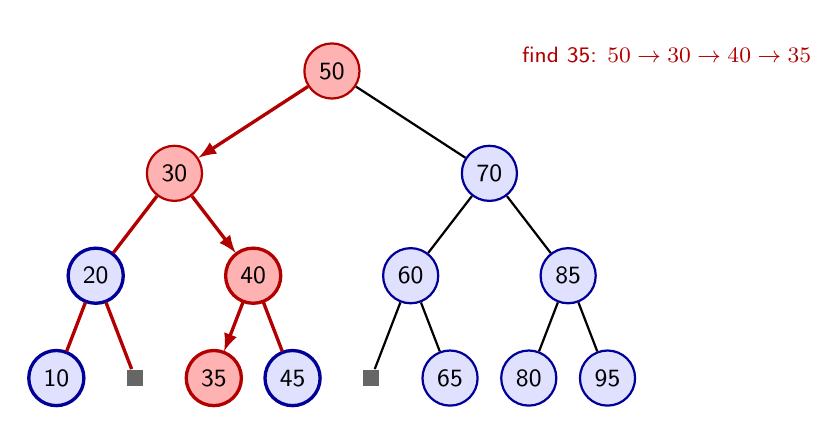
\begin{tikzpicture}[level distance=1.3cm, thick,
    level 1/.style={sibling distance=4cm},
    level 2/.style={sibling distance=2cm},
    level 3/.style={sibling distance=1cm},
    every node/.style={circle, draw=blue!60!black, fill=blue!12, minimum size=7mm, inner sep=0pt, font=\sffamily\small},
    found/.style={fill=red!30, draw=red!70!black},
    hit/.style={draw=red!70!black, very thick, -latex},
    nil/.style={rectangle, fill=black!60, draw=none, minimum size=2mm}]
  \node[found] {50}
    child { node[found] {30}
      child { node {20}
        child { node {10} }
        child { node[nil] {} } }
      child { node[found] {40}
        child { node[found] {35} edge from parent[hit] }
        child { node {45} }
        edge from parent[hit] }
      edge from parent[hit] }
    child { node {70}
      child { node {60}
        child { node[nil] {} }
        child { node {65} } }
      child { node {85}
        child { node {80} }
        child { node {95} } } };
  \node[rectangle, draw=none, fill=none, font=\sffamily\footnotesize, text=red!70!black, anchor=west] at (2.4,0.2) {find 35: $50 \to 30 \to 40 \to 35$};
\end{tikzpicture}
